\documentclass[10pt]{beamer}
\usetheme{metropolis}

% ── Packages ──
\usepackage{amsmath,amssymb,amsthm}
\usepackage{tikz}
\usetikzlibrary{positioning,arrows.meta,fit,matrix,backgrounds,calc}
\usepackage{graphicx}
\usepackage{array}
\usepackage{etoolbox}

% ── Theorem environments ──
\theoremstyle{definition}
\newtheorem{defi}{Definition}[section]
\newtheorem{prop}{Proposition}[section]
\newtheorem{thm}{Theorem}[section]
\newtheorem{cor}{Corollary}[section]

% Custom theorem styles with colors
\setbeamercolor{block title}{bg=red!75!black,fg=white}
\setbeamercolor{block body}{bg=yellow!10!white}

% Proposition uses yellow title
\AtBeginEnvironment{prop}{%
  \setbeamercolor{block title}{bg=yellow!75!black,fg=black}%
  \setbeamercolor{block body}{bg=yellow!10!white}%
}
\AtEndEnvironment{prop}{%
  \setbeamercolor{block title}{bg=red!75!black,fg=white}%
}

% Theorem uses yellow title
\AtBeginEnvironment{thm}{%
  \setbeamercolor{block title}{bg=yellow!75!black,fg=black}%
  \setbeamercolor{block body}{bg=yellow!10!white}%
}
\AtEndEnvironment{thm}{%
  \setbeamercolor{block title}{bg=red!75!black,fg=white}%
}

% ── Emoji definitions ──
\newcommand{\bean}{
\includegraphics[scale=0.07]{Pictures/bean.png}}
\newcommand{\leaf}{
\includegraphics[scale=0.08]{Pictures/leaf.png}}
\newcommand{\lemon}{
\includegraphics[scale=0.08]{Pictures/lemon.png}}
\newcommand{\cow}{
\includegraphics[scale=0.08]{Pictures/cow.png}}
\newcommand{\milk}{
\includegraphics[scale=0.08]{Pictures/milk.png}}
\newcommand{\coffee}{
\includegraphics[scale=0.08]{Pictures/coffee.png}}
\newcommand{\tea}{
\includegraphics[scale=0.08]{Pictures/tea.png}}
\newcommand{\bento}{
\includegraphics[scale=0.08]{Pictures/bento.png}}
\newcommand{\ramen}{\includegraphics[scale=0.08]{Pictures/ramen.png}}
\newcommand{\cola}{
\includegraphics[scale=0.08]{Pictures/cola.png}}

% ── Highlighting ──
\newcommand{\x}[1]{\alert{\textbf{#1}}}

\title{Lecture 5: Solving Linear Equations and Null Space}
\subtitle{MATH203 Applied Linear Algebra}
\date{}

\begin{document}
\maketitle

% ═══════════════════════════════════════
% §0 MOTIVATION
% ═══════════════════════════════════════
\section{Motivation: Why We Need to Solve Equations}

\begin{frame}{Recall: The Two Languages (Lecture 4)}

Every subspace has \x{two complementary descriptions}:

\vspace{1em}

\begin{center}
\begin{tabular}{|c|c|c|}
\hline
\textbf{Language} & \textbf{How it works} & \textbf{Example} \\
\hline
\x{Descriptive} & List \textbf{equations} & $\{\mathbf{x} : A\mathbf{x} = \mathbf{0}\}$ \\
 & (constraints) & \\
\hline
\x{Constructive} & Provide \textbf{recipe} & $\text{span}\{\mathbf{v}_1, \mathbf{v}_2, \ldots\}$ \\
 & (generate members) & \\
\hline
\end{tabular}
\end{center}

\vspace{1em}

\x{Today's question}: What is each language \textbf{good at}? What is each language \textbf{bad at}?

\end{frame}

\begin{frame}{Each Language Has Strengths and Weaknesses}

\begin{center}
\begin{tabular}{|c|c|c|}
\hline
& \x{Descriptive} & \x{Constructive} \\
& $\{\mathbf{x} : A\mathbf{x} = \mathbf{0}\}$ & $\text{span}\{\mathbf{v}_1, \ldots\}$ \\
\hline
\textbf{Generation} & Hard & \x{Easy} \\
(make a member) & Can't tell which $\mathbf{x}$ works & Just pick coefficients \\
\hline
\textbf{Verification} & \x{Easy} & Hard \\
(check membership) & Just compute $A\mathbf{x}$ & Solve equation \\
\hline
\end{tabular}
\end{center}

\vspace{1em}

\x{Goal of this lecture}: Learn to \textbf{solve equations} so we can:
\begin{itemize}
\item Convert descriptive $\to$ constructive (generation power)
\item Convert constructive $\to$ descriptive (verification power)
\end{itemize}

\end{frame}

% ═══════════════════════════════════════
% §1 CONCRETE EXAMPLE: FINDING NULL SPACE
% ═══════════════════════════════════════
\section{Concrete Example: Finding Null Space}

\begin{frame}{Example Setup: Shinchan's Coffee Shop Menu}

Shinchan has three drinks on his menu:

\vspace{0.5em}

\begin{center}
\begin{tabular}{c|ccc}
& \milk{} milk & \coffee{} coffee & \tea{} tea \\
\hline
\leaf{} tea leaves & 0 & 0 & 2 \\
\lemon{} lemon & 0 & 0 & 1 \\
\bean{} beans & 0 & 2 & 4 \\
\cow{} milk & 1 & 0 & 1 \\
\end{tabular}
\end{center}

\vspace{0.5em}

Matrix form:
$$\underbrace{\begin{pmatrix}
0 & 0 & 2 \\
0 & 0 & 1 \\
0 & 2 & 4 \\
1 & 0 & 1
\end{pmatrix}}_{A}$$

\end{frame}

\begin{frame}{The Question We Want to Answer}

\x{Question in coffee shop language}: \textbf{Which drinks can be made from other drinks?}

\vspace{1em}

For example:
\begin{itemize}
\item Can \tea{} be made from some combination of \milk{} and \coffee?
\item If so, what is the recipe?
\end{itemize}

\vspace{1em}

\x{Mathematical translation}: We're looking for \textbf{relationships between the columns} of $A$.

\vspace{0.5em}

If there's a relationship like ``2 coffees = 1 tea'', this means:

$$2 \times \begin{pmatrix} 0\\0\\2\\0 \end{pmatrix} = 1 \times \begin{pmatrix} 2\\1\\4\\1 \end{pmatrix}$$

which rearranges to: $0 \times \text{(milk)} + 2 \times \text{(coffee)} - 1 \times \text{(tea)} = \mathbf{0}$

\end{frame}

\begin{frame}{Setup: The Equation to Solve}

We're looking for all vectors $\mathbf{x} = \begin{pmatrix} x_1 \\ x_2 \\ x_3 \end{pmatrix}$ such that:

$$\underbrace{\begin{pmatrix}
0 & 0 & 2 \\
0 & 0 & 1 \\
0 & 2 & 4 \\
1 & 0 & 1
\end{pmatrix}}_{A} \begin{pmatrix} x_1 \\ x_2 \\ x_3 \end{pmatrix} = \begin{pmatrix} 0 \\ 0 \\ 0 \\ 0 \end{pmatrix}$$

\vspace{1em}

\x{Strategy}: Use \textbf{cross-filling} to decompose the augmented matrix $\underbrace{(A \mid \mathbf{0})}_{4 \times 4}$ into rank-one pieces, then solve backwards.

\end{frame}

\begin{frame}[fragile]{Step 1: Form Augmented Matrix}

\begin{center}
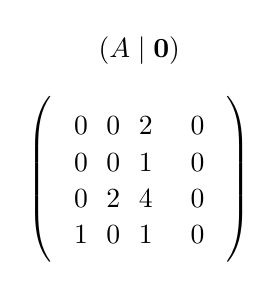
\begin{tikzpicture}[scale=0.7]
\matrix (m) [matrix of math nodes, left delimiter=(, right delimiter=), ampersand replacement=\&] {
0 \& 0 \& 2 \& \vrule \& 0 \\
0 \& 0 \& 1 \& \vrule \& 0 \\
0 \& 2 \& 4 \& \vrule \& 0 \\
1 \& 0 \& 1 \& \vrule \& 0 \\
};
\node[above=0.3cm of m] {$(A \mid \mathbf{0})$};
\end{tikzpicture}
\end{center}

\vspace{1em}

\x{Goal}: Cross-fill to find rank-one pieces $(R_i \mid \mathbf{b}_i)$.

\vspace{0.5em}

\x{First step}: Choose a pivot to start elimination.

\end{frame}

\begin{frame}[fragile]{Step 2: Choose First Pivot at (4,1)}

\begin{center}
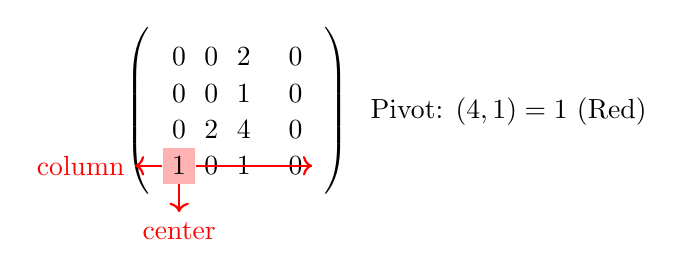
\begin{tikzpicture}[scale=0.7]
\matrix (m) [matrix of math nodes, left delimiter=(, right delimiter=), ampersand replacement=\&] {
0 \& 0 \& 2 \& \vrule \& 0 \\
0 \& 0 \& 1 \& \vrule \& 0 \\
0 \& 2 \& 4 \& \vrule \& 0 \\
|[fill=red!30]| 1 \& 0 \& 1 \& \vrule \& 0 \\
};
\draw[red, thick, ->] (m-4-1.south) -- ++(0, -0.5) node[below] {center};
\draw[red, thick, ->] (m-4-1.west) -- ++(-0.5, 0) node[left] {column};
\draw[red, thick, ->] (m-4-1.east) -- (m-4-5.east);
\node[right=0.5cm of m] {Pivot: $(4,1) = 1$ (Red)};
\end{tikzpicture}
\end{center}

\vspace{1em}

\x{Cross-filling formula}:

$$\underbrace{(R_1 \mid \mathbf{b}_1)}_{\text{rank-one}} = \underbrace{\frac{\text{column 1}}{1}}_{\text{normalized column}} \cdot (\text{row 4})$$

\end{frame}

\begin{frame}[fragile]{Step 3: Extract First Rank-One Piece}

\begin{center}
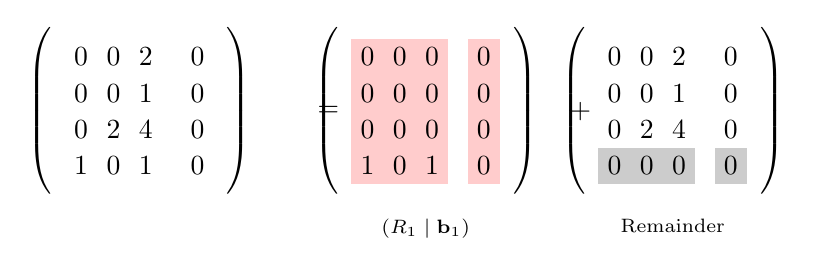
\begin{tikzpicture}[scale=0.8]
\matrix (m1) [matrix of math nodes, left delimiter=(, right delimiter=), ampersand replacement=\&] {
0 \& 0 \& 2 \& \vrule \& 0 \\
0 \& 0 \& 1 \& \vrule \& 0 \\
0 \& 2 \& 4 \& \vrule \& 0 \\
1 \& 0 \& 1 \& \vrule \& 0 \\
};
\node at (3, 0) {$=$};
\matrix (m2) [right=1.5cm of m1, matrix of math nodes, left delimiter=(, right delimiter=), ampersand replacement=\&] {
|[fill=red!20]| 0 \& |[fill=red!20]| 0 \& |[fill=red!20]| 0 \& \vrule \& |[fill=red!20]| 0 \\
|[fill=red!20]| 0 \& |[fill=red!20]| 0 \& |[fill=red!20]| 0 \& \vrule \& |[fill=red!20]| 0 \\
|[fill=red!20]| 0 \& |[fill=red!20]| 0 \& |[fill=red!20]| 0 \& \vrule \& |[fill=red!20]| 0 \\
|[fill=red!20]| 1 \& |[fill=red!20]| 0 \& |[fill=red!20]| 1 \& \vrule \& |[fill=red!20]| 0 \\
};
\node at (7, 0) {$+$};
\matrix (m3) [right=1cm of m2, matrix of math nodes, left delimiter=(, right delimiter=), ampersand replacement=\&] {
0 \& 0 \& 2 \& \vrule \& 0 \\
0 \& 0 \& 1 \& \vrule \& 0 \\
0 \& 2 \& 4 \& \vrule \& 0 \\
|[fill=gray!40]| 0 \& |[fill=gray!40]| 0 \& |[fill=gray!40]| 0 \& \vrule \& |[fill=gray!40]| 0 \\
};
\node[below=0.2cm of m2] {\scriptsize $(R_1 \mid \mathbf{b}_1)$};
\node[below=0.2cm of m3] {\scriptsize Remainder};
\end{tikzpicture}
\end{center}

\vspace{0.5em}

\x{Observation}: Column 1 is now eliminated from the remainder!

\end{frame}

\begin{frame}[fragile]{Step 4: Choose Second Pivot at (3,2)}

\begin{center}
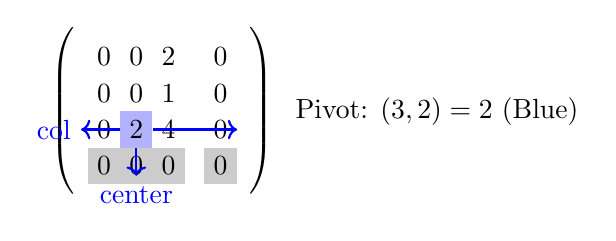
\begin{tikzpicture}[scale=0.7]
\matrix (m) [matrix of math nodes, left delimiter=(, right delimiter=), ampersand replacement=\&] {
0 \& 0 \& 2 \& \vrule \& 0 \\
0 \& 0 \& 1 \& \vrule \& 0 \\
0 \& |[fill=blue!30]| 2 \& 4 \& \vrule \& 0 \\
|[fill=gray!40]| 0 \& |[fill=gray!40]| 0 \& |[fill=gray!40]| 0 \& \vrule \& |[fill=gray!40]| 0 \\
};
\draw[blue, thick, ->] (m-3-2.south) -- ++(0, -0.5) node[below] {center};
\draw[blue, thick, ->] (m-3-2.west) -- ++(-0.7, 0) node[left] {col};
\draw[blue, thick, ->] (m-3-2.east) -- (m-3-5.east);
\node[right=0.5cm of m] {Pivot: $(3,2) = 2$ (Blue)};
\end{tikzpicture}
\end{center}

\vspace{1em}

\x{Cross-filling formula}:

$$\underbrace{(R_2 \mid \mathbf{b}_2)}_{\text{rank-one}} = \underbrace{\frac{\text{column 2 of remainder}}{2}}_{\text{normalized column}} \cdot (\text{row 3 of remainder})$$

\vspace{0.5em}

Note: Column 2 of remainder = $\begin{pmatrix} 0 \\ 0 \\ 2 \\ 0 \end{pmatrix}$ (column 1 already zero)

\end{frame}

\begin{frame}[fragile]{Step 5: Extract Second Rank-One Piece}

\begin{center}
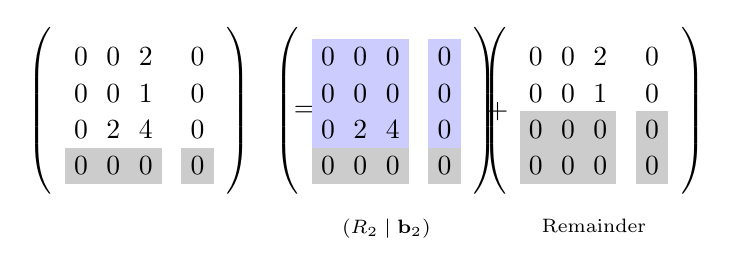
\begin{tikzpicture}[scale=0.7]
\matrix (m1) [matrix of math nodes, left delimiter=(, right delimiter=), ampersand replacement=\&] {
0 \& 0 \& 2 \& \vrule \& 0 \\
0 \& 0 \& 1 \& \vrule \& 0 \\
0 \& 2 \& 4 \& \vrule \& 0 \\
|[fill=gray!40]| 0 \& |[fill=gray!40]| 0 \& |[fill=gray!40]| 0 \& \vrule \& |[fill=gray!40]| 0 \\
};
\node at (3, 0) {$=$};
\matrix (m2) [right=1cm of m1, matrix of math nodes, left delimiter=(, right delimiter=), ampersand replacement=\&] {
|[fill=blue!20]| 0 \& |[fill=blue!20]| 0 \& |[fill=blue!20]| 0 \& \vrule \& |[fill=blue!20]| 0 \\
|[fill=blue!20]| 0 \& |[fill=blue!20]| 0 \& |[fill=blue!20]| 0 \& \vrule \& |[fill=blue!20]| 0 \\
|[fill=blue!20]| 0 \& |[fill=blue!20]| 2 \& |[fill=blue!20]| 4 \& \vrule \& |[fill=blue!20]| 0 \\
|[fill=gray!40]| 0 \& |[fill=gray!40]| 0 \& |[fill=gray!40]| 0 \& \vrule \& |[fill=gray!40]| 0 \\
};
\node at (6.5, 0) {$+$};
\matrix (m3) [right=0.5cm of m2, matrix of math nodes, left delimiter=(, right delimiter=), ampersand replacement=\&] {
0 \& 0 \& 2 \& \vrule \& 0 \\
0 \& 0 \& 1 \& \vrule \& 0 \\
|[fill=gray!40]| 0 \& |[fill=gray!40]| 0 \& |[fill=gray!40]| 0 \& \vrule \& |[fill=gray!40]| 0 \\
|[fill=gray!40]| 0 \& |[fill=gray!40]| 0 \& |[fill=gray!40]| 0 \& \vrule \& |[fill=gray!40]| 0 \\
};
\node[below=0.2cm of m2] {\scriptsize $(R_2 \mid \mathbf{b}_2)$};
\node[below=0.2cm of m3] {\scriptsize Remainder};
\end{tikzpicture}
\end{center}

\vspace{0.5em}

\x{Observation}: Columns 1 and 2 are now eliminated! Remainder only has column 3 active.

\end{frame}

\begin{frame}[fragile]{Step 6: Choose Third Pivot at (1,3)}

\begin{center}
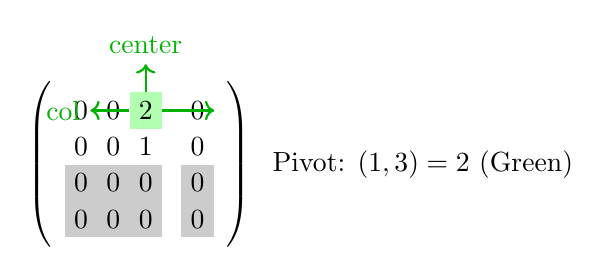
\begin{tikzpicture}[scale=0.7]
\matrix (m) [matrix of math nodes, left delimiter=(, right delimiter=), ampersand replacement=\&] {
0 \& 0 \& |[fill=green!30]| 2 \& \vrule \& 0 \\
0 \& 0 \& 1 \& \vrule \& 0 \\
|[fill=gray!40]| 0 \& |[fill=gray!40]| 0 \& |[fill=gray!40]| 0 \& \vrule \& |[fill=gray!40]| 0 \\
|[fill=gray!40]| 0 \& |[fill=gray!40]| 0 \& |[fill=gray!40]| 0 \& \vrule \& |[fill=gray!40]| 0 \\
};
\draw[green!70!black, thick, ->] (m-1-3.north) -- ++(0, 0.5) node[above] {center};
\draw[green!70!black, thick, ->] (m-1-3.west) -- ++(-0.7, 0) node[left] {col};
\draw[green!70!black, thick, ->] (m-1-3.east) -- (m-1-5.east);
\node[right=0.5cm of m] {Pivot: $(1,3) = 2$ (Green)};
\end{tikzpicture}
\end{center}

\vspace{1em}

\x{Cross-filling formula}:

$$\underbrace{(R_3 \mid \mathbf{b}_3)}_{\text{rank-one}} = \underbrace{\frac{\text{column 3 of remainder}}{2}}_{\text{normalized column}} \cdot (\text{row 1 of remainder})$$

\end{frame}

\begin{frame}[fragile]{Step 7: Complete Decomposition}

\begin{center}
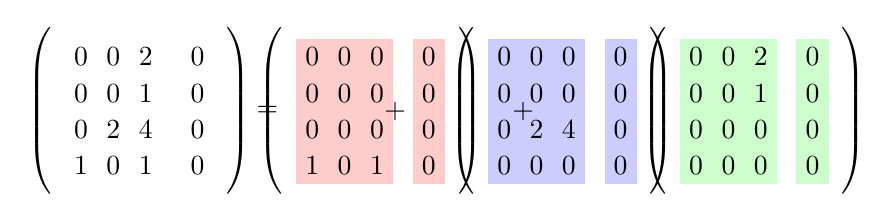
\begin{tikzpicture}[scale=0.65]
\matrix (m0) [matrix of math nodes, left delimiter=(, right delimiter=), ampersand replacement=\&] {
0 \& 0 \& 2 \& \vrule \& 0 \\
0 \& 0 \& 1 \& \vrule \& 0 \\
0 \& 2 \& 4 \& \vrule \& 0 \\
1 \& 0 \& 1 \& \vrule \& 0 \\
};
\node at (2.5, 0) {$=$};
\matrix (m1) [right=0.8cm of m0, matrix of math nodes, left delimiter=(, right delimiter=), ampersand replacement=\&] {
|[fill=red!20]| 0 \& |[fill=red!20]| 0 \& |[fill=red!20]| 0 \& \vrule \& |[fill=red!20]| 0 \\
|[fill=red!20]| 0 \& |[fill=red!20]| 0 \& |[fill=red!20]| 0 \& \vrule \& |[fill=red!20]| 0 \\
|[fill=red!20]| 0 \& |[fill=red!20]| 0 \& |[fill=red!20]| 0 \& \vrule \& |[fill=red!20]| 0 \\
|[fill=red!20]| 1 \& |[fill=red!20]| 0 \& |[fill=red!20]| 1 \& \vrule \& |[fill=red!20]| 0 \\
};
\node at (5, 0) {$+$};
\matrix (m2) [right=0.3cm of m1, matrix of math nodes, left delimiter=(, right delimiter=), ampersand replacement=\&] {
|[fill=blue!20]| 0 \& |[fill=blue!20]| 0 \& |[fill=blue!20]| 0 \& \vrule \& |[fill=blue!20]| 0 \\
|[fill=blue!20]| 0 \& |[fill=blue!20]| 0 \& |[fill=blue!20]| 0 \& \vrule \& |[fill=blue!20]| 0 \\
|[fill=blue!20]| 0 \& |[fill=blue!20]| 2 \& |[fill=blue!20]| 4 \& \vrule \& |[fill=blue!20]| 0 \\
|[fill=blue!20]| 0 \& |[fill=blue!20]| 0 \& |[fill=blue!20]| 0 \& \vrule \& |[fill=blue!20]| 0 \\
};
\node at (7.5, 0) {$+$};
\matrix (m3) [right=0.3cm of m2, matrix of math nodes, left delimiter=(, right delimiter=), ampersand replacement=\&] {
|[fill=green!20]| 0 \& |[fill=green!20]| 0 \& |[fill=green!20]| 2 \& \vrule \& |[fill=green!20]| 0 \\
|[fill=green!20]| 0 \& |[fill=green!20]| 0 \& |[fill=green!20]| 1 \& \vrule \& |[fill=green!20]| 0 \\
|[fill=green!20]| 0 \& |[fill=green!20]| 0 \& |[fill=green!20]| 0 \& \vrule \& |[fill=green!20]| 0 \\
|[fill=green!20]| 0 \& |[fill=green!20]| 0 \& |[fill=green!20]| 0 \& \vrule \& |[fill=green!20]| 0 \\
};
\end{tikzpicture}
\end{center}

\vspace{1em}

$$(A \mid \mathbf{0}) = \underbrace{(R_1 \mid \mathbf{b}_1)}_{\text{Red}} + \underbrace{(R_2 \mid \mathbf{b}_2)}_{\text{Blue}} + \underbrace{(R_3 \mid \mathbf{b}_3)}_{\text{Green}}$$

\vspace{0.5em}

\x{Next}: Read off the simplified equations from each piece!

\end{frame}

\begin{frame}{Step 8: Read Off Simplified Equations}

Each rank-one piece gives one simplified equation:

\vspace{1em}

\x{From $(R_1 \mid \mathbf{b}_1)$} (row 4):
$$1 \cdot x_1 + 0 \cdot x_2 + 1 \cdot x_3 = 0 \quad \Rightarrow \quad \boxed{x_1 + x_3 = 0}$$

\vspace{0.5em}

\x{From $(R_2 \mid \mathbf{b}_2)$} (row 3):
$$0 \cdot x_1 + 2 \cdot x_2 + 4 \cdot x_3 = 0 \quad \Rightarrow \quad \boxed{2x_2 + 4x_3 = 0}$$

\vspace{0.5em}

\x{From $(R_3 \mid \mathbf{b}_3)$} (rows 1,2):
$$\begin{cases}
0 \cdot x_1 + 0 \cdot x_2 + 2 \cdot x_3 = 0 \\
0 \cdot x_1 + 0 \cdot x_2 + 1 \cdot x_3 = 0
\end{cases} \quad \Rightarrow \quad \boxed{x_3 = 0}$$

\vspace{1em}

\x{Key observation}: Each equation involves \textbf{fewer variables} than the previous!

\end{frame}

\begin{frame}{Step 9: Solve Backwards}

We have three equations with decreasing complexity:

\vspace{0.5em}

\begin{enumerate}
\item From $(R_3 \mid \mathbf{b}_3)$: $x_3 = 0$
\item From $(R_2 \mid \mathbf{b}_2)$: $2x_2 + 4x_3 = 0$
\item From $(R_1 \mid \mathbf{b}_1)$: $x_1 + x_3 = 0$
\end{enumerate}

\vspace{1em}

\x{Solve backwards} (start from the simplest):

\begin{align*}
x_3 &= 0 \quad \text{(from equation 1)} \\
2x_2 + 4(0) &= 0 \quad \Rightarrow \quad x_2 = 0 \quad \text{(from equation 2)} \\
x_1 + 0 &= 0 \quad \Rightarrow \quad x_1 = 0 \quad \text{(from equation 3)}
\end{align*}

\vspace{1em}

\x{Conclusion}: The only solution is $\mathbf{x} = \begin{pmatrix} 0 \\ 0 \\ 0 \end{pmatrix}$.

\end{frame}

\begin{frame}{Step 10: Interpret the Answer}

\x{Mathematical conclusion}: The null space is:

$$\text{Null}(A) = \{\mathbf{0}\}$$

\vspace{1em}

\x{Coffee shop interpretation}: There are \textbf{NO non-trivial relationships} between the drinks!

\vspace{0.5em}

\begin{itemize}
\item \tea{} cannot be made from \milk{} and \coffee
\item \milk{} cannot be made from \coffee{} and \tea
\item \coffee{} cannot be made from \milk{} and \tea
\end{itemize}

\vspace{1em}

All three drinks are \x{linearly independent} $\Rightarrow$ no drink is redundant!

\end{frame}

\begin{frame}{What We Just Did}

\x{Summary of the cross-filling method}:

\begin{enumerate}
\item Form augmented matrix $\underbrace{(A \mid \mathbf{0})}_{m \times (n+1)}$
\item Decompose into rank-one pieces: $(A \mid \mathbf{0}) = (R_1 \mid \mathbf{b}_1) + (R_2 \mid \mathbf{b}_2) + \cdots$
\item Each piece gives a simplified equation
\item Variables decrease with each step
\item Solve backwards from simplest to most complex
\end{enumerate}

\vspace{1em}

\x{Now we formalize}: What did we actually find? What is "null space"?

\end{frame}

% ═══════════════════════════════════════
% §1.5 FORMALIZE: NULL SPACE DEFINITION
% ═══════════════════════════════════════

\begin{frame}{Null Space: Definition (Extracted from Example)}

\begin{defi}[Null Space (Kernel)]
For a matrix $\underbrace{A}_{m \times n}$, the \x{null space} is:

$$\text{Null}(A) = \{\mathbf{x} \in \mathbb{R}^n : A\mathbf{x} = \mathbf{0}\}$$

\textbf{Meaning}: $\text{Null}(A)$ records all \x{relationships between the columns} of $A$.

Also called the \x{kernel}, denoted $\ker(A)$.
\end{defi}

\vspace{0.5em}

\x{In coffee shop language}: Drink combinations that reveal "which drinks can be made from others."

\vspace{0.5em}

\x{In our example}: $\text{Null}(A) = \{\mathbf{0}\}$ means no drink can be made from others.

\end{frame}

\begin{frame}{Why Augmented Matrix $(A \mid \mathbf{0})$?}

\x{Question}: Why did we form $(A \mid \mathbf{0})$ instead of just working with $A$?

\vspace{1em}

\x{Answer}: The augmented matrix tracks the \textbf{right-hand side} of the equation!

\vspace{0.5em}

For $A\mathbf{x} = \mathbf{b}$, we need to track both:
\begin{itemize}
\item The coefficients (left side): $\underbrace{A}_{m \times n}$
\item The target values (right side): $\underbrace{\mathbf{b}}_{m \times 1}$
\end{itemize}

\vspace{1em}

Augmented matrix: $\underbrace{(A \mid \mathbf{b})}_{m \times (n+1)}$ keeps them together!

\vspace{0.5em}

\x{For null space}: $\mathbf{b} = \mathbf{0}$, so we use $\underbrace{(A \mid \mathbf{0})}_{m \times (n+1)}$.

\end{frame}

\begin{frame}{Connection: Null Space vs Column Space}

Recall from motivation:

\begin{center}
\begin{tabular}{|c|c|c|}
\hline
\textbf{Subspace} & \textbf{Natural form} & \textbf{What it records} \\
\hline
$\text{Col}(A)$ & Constructive & All combinations of columns \\
 & span$\{$ columns $\}$ & (what we can make) \\
\hline
$\text{Null}(A)$ & Descriptive & Relationships between columns \\
 & $\{\mathbf{x} : A\mathbf{x} = \mathbf{0}\}$ & (which are redundant) \\
\hline
\end{tabular}
\end{center}

\vspace{1em}

\x{Connection}: If $\text{Null}(A) = \{\mathbf{0}\}$, then:
\begin{itemize}
\item No column can be made from others
\item All columns are linearly independent
\item $\text{Col}(A)$ has dimension = number of columns
\end{itemize}

\end{frame}

% ═══════════════════════════════════════
% §2 WHY CROSS-FILLING WORKS
% ═══════════════════════════════════════
\section{Why Cross-Filling Works}

\begin{frame}{Look Back at What We Did}

In the example, we decomposed:

$$\underbrace{(A \mid \mathbf{0})}_{4 \times 4} = \underbrace{(R_1 \mid \mathbf{b}_1)}_{\text{Red}} + \underbrace{(R_2 \mid \mathbf{b}_2)}_{\text{Blue}} + \underbrace{(R_3 \mid \mathbf{b}_3)}_{\text{Green}}$$

\vspace{1em}

\x{Each piece gave us a simplified equation}:
\begin{itemize}
\item $(R_1 \mid \mathbf{b}_1)$ had only $x_1, x_3$ active (from row 4)
\item $(R_2 \mid \mathbf{b}_2)$ had only $x_2, x_3$ active (from row 3)
\item $(R_3 \mid \mathbf{b}_3)$ had only $x_3$ active (from rows 1,2)
\end{itemize}

\vspace{1em}

\x{Question}: \textbf{Why} does each piece give a simplified equation? What's the underlying principle?

\end{frame}

\begin{frame}{Principle 1: Each Piece = One Equation}

Each rank-one piece $\underbrace{(R_i \mid \mathbf{b}_i)}_{m \times (n+1)}$ represents \x{one equation}.

\vspace{1em}

\x{Why?} Rank-one means:

$$(R_i \mid \mathbf{b}_i) = \underbrace{\mathbf{u}}_{m \times 1} \cdot \underbrace{\mathbf{v}^T}_{1 \times (n+1)}$$

where $\mathbf{u} =$ column (normalized pivot column) and $\mathbf{v}^T =$ row (pivot row).

\vspace{1em}

\x{In our red piece}:

$$\underbrace{\begin{pmatrix} 0\\0\\0\\1 \end{pmatrix}}_{\mathbf{u}} \cdot \underbrace{\begin{pmatrix} 0 & 0 & 0 & \mid & 0 \\ 0 & 0 & 1 & \mid & 0 \end{pmatrix}}_{\text{actually just row 4: } \begin{pmatrix} 1 & 0 & 1 & \mid & 0 \end{pmatrix}}$$

Wait, let me correct this...

\end{frame}

\begin{frame}{Principle 1: Each Piece = One Equation (Corrected)}

Each rank-one piece gives ONE equation from the \textbf{pivot row}.

\vspace{1em}

\x{From our example} (Red piece, pivot row 4):

$$\underbrace{(R_1 \mid \mathbf{b}_1)}_{\text{rank-one}} = \text{only row 4 is non-zero: } \begin{pmatrix} 1 & 0 & 1 & \mid & 0 \end{pmatrix}$$

This says: $1 \cdot x_1 + 0 \cdot x_2 + 1 \cdot x_3 = 0$, i.e., $\boxed{x_1 + x_3 = 0}$.

\vspace{1em}

\x{From our example} (Blue piece, pivot row 3):

$$\underbrace{(R_2 \mid \mathbf{b}_2)}_{\text{rank-one}} = \text{only row 3 is non-zero: } \begin{pmatrix} 0 & 2 & 4 & \mid & 0 \end{pmatrix}$$

This says: $0 \cdot x_1 + 2 \cdot x_2 + 4 \cdot x_3 = 0$, i.e., $\boxed{2x_2 + 4x_3 = 0}$.

\end{frame}

\begin{frame}{Principle 2: Variables Decrease}

As cross-filling proceeds, each piece has \textbf{fewer active variables}.

\vspace{1em}

\x{In our example}:

\begin{center}
\begin{tabular}{|c|c|c|}
\hline
\textbf{Piece} & \textbf{Pivot row equation} & \textbf{Active variables} \\
\hline
$(R_1 \mid \mathbf{b}_1)$ & $x_1 + x_3 = 0$ & $x_1, x_3$ (2 vars) \\
\hline
$(R_2 \mid \mathbf{b}_2)$ & $2x_2 + 4x_3 = 0$ & $x_2, x_3$ (2 vars) \\
\hline
$(R_3 \mid \mathbf{b}_3)$ & $x_3 = 0$ & $x_3$ (1 var) \\
\hline
\end{tabular}
\end{center}

\vspace{1em}

\x{General principle}: After eliminating column $j_i$ with pivot, \textbf{at least column $j_i$ is gone} from the remainder (possibly more columns eliminated together).

\vspace{0.5em}

$\Rightarrow$ Each successive piece has \textbf{at least one fewer variable}.

\end{frame}

\begin{frame}{Principle 3: V Matrix Collects Simplified Equations}

Stack all the pivot rows to form the $\x{V}$ matrix:

$$V = \begin{pmatrix}
\text{— row from } (R_1 \mid \mathbf{b}_1) \text{ —} \\
\text{— row from } (R_2 \mid \mathbf{b}_2) \text{ —} \\
\vdots \\
\text{— row from } (R_r \mid \mathbf{b}_r) \text{ —}
\end{pmatrix}$$

\vspace{1em}

\x{In our example} (3 pivot rows):

$$V = \begin{pmatrix}
1 & 0 & 1 & \mid & 0 \\
0 & 2 & 4 & \mid & 0 \\
0 & 0 & 2 & \mid & 0
\end{pmatrix}$$

\vspace{0.5em}

Each row = one simplified equation!

\end{frame}

\begin{frame}{Principle 4: Left Cancellation (Why $V$ is Equivalent to $A$)}

\x{Key question}: Why is solving $V\mathbf{x} = \mathbf{0}$ the same as solving $A\mathbf{x} = \mathbf{0}$?

\vspace{1em}

\x{Answer}: Because $(A \mid \mathbf{0}) = (R_1 \mid \mathbf{b}_1) + \cdots + (R_r \mid \mathbf{b}_r)$.

\vspace{0.5em}

This means:

$$\underbrace{A}_{m \times n} \mathbf{x} = \underbrace{R_1 + \cdots + R_r}_{m \times n} \mathbf{x}$$

\vspace{1em}

Each $R_i$ is rank-one: $R_i = \mathbf{u}_i \mathbf{v}_i^T$ where $\mathbf{v}_i^T$ is the $i$-th row of $V$.

$$R_i \mathbf{x} = \mathbf{u}_i (\mathbf{v}_i^T \mathbf{x})$$

So: $A\mathbf{x} = \sum_{i=1}^r \mathbf{u}_i (\mathbf{v}_i^T \mathbf{x}) = \underbrace{U}_{m \times r} \underbrace{V}_{r \times n} \mathbf{x}$

\end{frame}

\begin{frame}{Left Cancellation: $UV\mathbf{x} = \mathbf{0} \iff V\mathbf{x} = \mathbf{0}$}

We have: $\underbrace{A}_{m \times n} = \underbrace{U}_{m \times r} \underbrace{V}_{r \times n}$

\vspace{1em}

\x{Question}: Does $A\mathbf{x} = \mathbf{0}$ imply $V\mathbf{x} = \mathbf{0}$?

\vspace{0.5em}

\x{Answer}: YES! By left cancellation:

\begin{align*}
UV\mathbf{x} &= \mathbf{0} \\
\iff UV\mathbf{x} &= U\mathbf{0} \quad \text{(since $U\mathbf{0} = \mathbf{0}$)} \\
\iff V\mathbf{x} &= \mathbf{0} \quad \text{(left cancel $U$ if columns of $U$ are linearly independent)}
\end{align*}

\vspace{1em}

\x{Why can we cancel $U$?} Because $U$ has rank $r$ (full column rank) $\Rightarrow$ its columns are linearly independent!

\end{frame}

\begin{frame}{Explicit $U$ and $V$ in Our Example}

From our cross-filling:

$$U = \begin{pmatrix}
| & | & | \\
\mathbf{u}_1 & \mathbf{u}_2 & \mathbf{u}_3 \\
| & | & |
\end{pmatrix} = \begin{pmatrix}
0 & 0 & 1 \\
0 & 0 & \frac{1}{2} \\
0 & 1 & 0 \\
1 & 0 & 0
\end{pmatrix}$$

$$V = \begin{pmatrix}
- & \mathbf{v}_1^T & - \\
- & \mathbf{v}_2^T & - \\
- & \mathbf{v}_3^T & -
\end{pmatrix} = \begin{pmatrix}
1 & 0 & 1 \\
0 & 2 & 4 \\
0 & 0 & 2
\end{pmatrix}$$

\vspace{0.5em}

Check: $UV = A$ and $\underbrace{V}_{3 \times 3} \mathbf{x} = \mathbf{0}$ gives the simplified system!

\end{frame}

\begin{frame}{Summary: Why Cross-Filling Works}

\x{Four key principles}:

\begin{enumerate}
\item \textbf{Each rank-one piece = one equation} (from the pivot row)
\item \textbf{Variables decrease} (at least one variable eliminated per step)
\item \textbf{$V$ matrix collects all simplified equations} (stack pivot rows)
\item \textbf{Left cancellation}: $A = UV$ and $UV\mathbf{x} = \mathbf{0} \iff V\mathbf{x} = \mathbf{0}$
\end{enumerate}

\vspace{1em}

\x{Result}: Solving $\underbrace{A}_{m \times n}\mathbf{x} = \mathbf{0}$ reduces to solving $\underbrace{V}_{r \times n}\mathbf{x} = \mathbf{0}$ where $V$ has \textbf{simpler structure} (upper triangular with decreasing variables).

\vspace{0.5em}

$\Rightarrow$ Backward substitution becomes easy!

\end{frame}

\begin{frame}{General Cross-Filling Algorithm (Formalized)}

\x{Input}: $m \times n$ matrix $\underbrace{A}_{m \times n}$ and target $\underbrace{\mathbf{b}}_{m \times 1}$

\x{Output}: Solution to $A\mathbf{x} = \mathbf{b}$ (if exists)

\vspace{1em}

\x{Steps}:
\begin{enumerate}
\item Form augmented matrix $\underbrace{(A \mid \mathbf{b})}_{m \times (n+1)}$
\item Cross-fill: $(A \mid \mathbf{b}) = (R_1 \mid \mathbf{b}_1) + \cdots + (R_r \mid \mathbf{b}_r)$
\item Collect pivot rows into $V$ matrix (size $r \times (n+1)$)
\item Check each non-pivot row:
   \begin{itemize}
   \item If row $= \begin{pmatrix} 0 & \cdots & 0 & \mid & 0 \end{pmatrix}$ $\Rightarrow$ OK
   \item If row $= \begin{pmatrix} 0 & \cdots & 0 & \mid & c \end{pmatrix}$ with $c \neq 0$ $\Rightarrow$ NO solution!
   \end{itemize}
\item If all non-pivot rows are OK, solve $V\mathbf{x} = \mathbf{b}_V$ backwards
\end{enumerate}

\end{frame}

% ═══════════════════════════════════════
% §3 SOLVING GENERAL EQUATIONS
% ═══════════════════════════════════════
\section{Solving General Equations $A\mathbf{x} = \mathbf{b}$}

\begin{frame}{New Example: Non-Zero Right-Hand Side}

\x{Setup}: Solve $\underbrace{A}_{3 \times 4}\mathbf{x} = \underbrace{\mathbf{b}}_{3 \times 1}$ where

$$A = \begin{pmatrix}
1 & 2 & 0 & 1 \\
2 & 4 & 1 & 2 \\
3 & 6 & 1 & 3
\end{pmatrix}, \quad \mathbf{b} = \begin{pmatrix} 5 \\ 11 \\ 16 \end{pmatrix}$$

\vspace{1em}

\x{Difference from before}: Now $\mathbf{b} \neq \mathbf{0}$, so we're looking for \textbf{actual solutions} (not just relationships).

\vspace{0.5em}

\x{Method}: Same cross-filling, but track the right-hand side!

\end{frame}

\begin{frame}[fragile]{Cross-Filling with $\mathbf{b} \neq \mathbf{0}$}

Form augmented matrix and cross-fill (details similar to before):

\vspace{0.5em}

$$(A \mid \mathbf{b}) = \underbrace{(R_1 \mid \mathbf{b}_1)}_{\text{pivot (1,1)}} + \underbrace{(R_2 \mid \mathbf{b}_2)}_{\text{pivot (2,3)}}$$

\vspace{0.5em}

Collect pivot rows into $V$:

$$V = \begin{pmatrix}
1 & 2 & 0 & 1 & \mid & 5 \\
0 & 0 & 1 & 0 & \mid & 1
\end{pmatrix}$$

\vspace{1em}

\x{Equations from $V$}:
\begin{align*}
x_1 + 2x_2 + 0x_3 + 1x_4 &= 5 \\
0x_1 + 0x_2 + 1x_3 + 0x_4 &= 1
\end{align*}

\end{frame}

\begin{frame}{Identify Pivot and Free Variables}

From the $V$ matrix:

$$V = \begin{pmatrix}
1 & 2 & 0 & 1 & \mid & 5 \\
0 & 0 & 1 & 0 & \mid & 1
\end{pmatrix}$$

\vspace{1em}

\x{Pivot variables}: $x_1$ (from row 1), $x_3$ (from row 2)

\x{Free variables}: $x_2, x_4$ (columns without pivots)

\vspace{1em}

\x{Strategy}: Set free variables to arbitrary values, solve for pivot variables.

\end{frame}

\begin{frame}{Solve Backwards: Find One Particular Solution}

Set free variables to convenient values: $x_2 = 0, x_4 = 0$.

\vspace{1em}

\x{From equation 2}: $x_3 = 1$

\x{From equation 1}: $x_1 + 2(0) + 0(1) + 1(0) = 5 \Rightarrow x_1 = 5$

\vspace{1em}

\x{One particular solution}:

$$\mathbf{x}_p = \begin{pmatrix} 5 \\ 0 \\ 1 \\ 0 \end{pmatrix}$$

\vspace{0.5em}

Verify: $A\mathbf{x}_p = \begin{pmatrix} 5 \\ 11 \\ 16 \end{pmatrix} = \mathbf{b}$ \checkmark

\end{frame}

\begin{frame}{General Solution: Add Null Space}

\x{Question}: Are there other solutions besides $\mathbf{x}_p$?

\vspace{1em}

\x{Answer}: YES! Any $\mathbf{x} = \mathbf{x}_p + \mathbf{x}_n$ where $\mathbf{x}_n \in \text{Null}(A)$.

\vspace{0.5em}

\x{Why?}
\begin{align*}
A(\mathbf{x}_p + \mathbf{x}_n) &= A\mathbf{x}_p + A\mathbf{x}_n \\
&= \mathbf{b} + \mathbf{0} = \mathbf{b} \quad \checkmark
\end{align*}

\vspace{1em}

\x{To find all solutions}:
\begin{enumerate}
\item Find one particular solution $\mathbf{x}_p$ (set free vars = 0)
\item Find basis for $\text{Null}(A)$ (set each free var = 1, others = 0)
\item General solution: $\mathbf{x} = \mathbf{x}_p + c_1\mathbf{v}_1 + c_2\mathbf{v}_2 + \cdots$
\end{enumerate}

\end{frame}

\begin{frame}{Finding Null Space Basis (Concrete Example)}

From $V$:

$$V = \begin{pmatrix}
1 & 2 & 0 & 1 & \mid & 0 \\
0 & 0 & 1 & 0 & \mid & 0
\end{pmatrix}$$

Free variables: $x_2, x_4$. We need 2 basis vectors.

\vspace{1em}

\x{Vector 1}: Set $x_2 = 1, x_4 = 0$

\begin{align*}
x_3 &= 0 \quad \text{(from row 2)} \\
x_1 + 2(1) + 0(0) + 1(0) &= 0 \quad \Rightarrow \quad x_1 = -2 \quad \text{(from row 1)}
\end{align*}

$$\mathbf{v}_1 = \begin{pmatrix} -2 \\ 1 \\ 0 \\ 0 \end{pmatrix}$$

\end{frame}

\begin{frame}{Finding Null Space Basis (Continued)}

\x{Vector 2}: Set $x_2 = 0, x_4 = 1$

\begin{align*}
x_3 &= 0 \quad \text{(from row 2)} \\
x_1 + 2(0) + 0(0) + 1(1) &= 0 \quad \Rightarrow \quad x_1 = -1 \quad \text{(from row 1)}
\end{align*}

$$\mathbf{v}_2 = \begin{pmatrix} -1 \\ 0 \\ 0 \\ 1 \end{pmatrix}$$

\vspace{1em}

\x{Basis for $\text{Null}(A)$}:

$$\left\{ \begin{pmatrix} -2 \\ 1 \\ 0 \\ 0 \end{pmatrix}, \begin{pmatrix} -1 \\ 0 \\ 0 \\ 1 \end{pmatrix} \right\}$$

\end{frame}

\begin{frame}{Complete Solution Set}

\x{General solution to $A\mathbf{x} = \mathbf{b}$}:

$$\mathbf{x} = \underbrace{\begin{pmatrix} 5 \\ 0 \\ 1 \\ 0 \end{pmatrix}}_{\mathbf{x}_p} + c_1 \underbrace{\begin{pmatrix} -2 \\ 1 \\ 0 \\ 0 \end{pmatrix}}_{\mathbf{v}_1} + c_2 \underbrace{\begin{pmatrix} -1 \\ 0 \\ 0 \\ 1 \end{pmatrix}}_{\mathbf{v}_2}$$

where $c_1, c_2 \in \mathbb{R}$ are arbitrary.

\vspace{1em}

\x{Geometric picture}: The solution set is an \textbf{affine subspace}:

$$\text{Solutions} = \mathbf{x}_p + \text{Null}(A)$$

\vspace{0.5em}

(A 2-dimensional plane in $\mathbb{R}^4$ passing through $\mathbf{x}_p$)

\end{frame}

\begin{frame}{Existence: When Does $A\mathbf{x} = \mathbf{b}$ Have Solutions?}

Look at the cross-filling decomposition:

$$(A \mid \mathbf{b}) = (R_1 \mid \mathbf{b}_1) + \cdots + (R_r \mid \mathbf{b}_r)$$

\vspace{1em}

\x{Two cases for non-pivot rows}:

\begin{itemize}
\item \textbf{Case 1}: Non-pivot row = $\begin{pmatrix} 0 & \cdots & 0 & \mid & 0 \end{pmatrix}$

This is OK! Just says $0 = 0$ (always true).

\item \textbf{Case 2}: Non-pivot row = $\begin{pmatrix} 0 & \cdots & 0 & \mid & c \end{pmatrix}$ with $c \neq 0$

This is CONTRADICTION! Says $0 = c$ where $c \neq 0$ (impossible).
\end{itemize}

\vspace{1em}

\x{Conclusion}: Solution exists $\iff$ no Case 2 rows appear.

\end{frame}

\begin{frame}[fragile]{Visual: Existence Cases}

\begin{center}
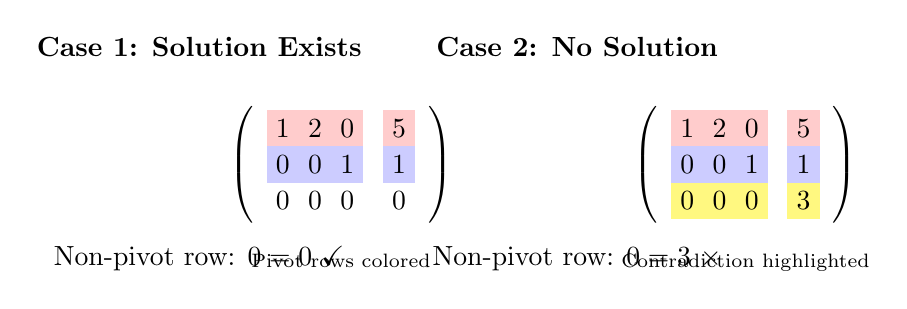
\begin{tikzpicture}[scale=0.6]
% Case 1
\node at (-3, 2.5) {\textbf{Case 1: Solution Exists}};
\matrix (m1) [matrix of math nodes, left delimiter=(, right delimiter=), ampersand replacement=\&] {
|[fill=red!20]| 1 \& |[fill=red!20]| 2 \& |[fill=red!20]| 0 \& \vrule \& |[fill=red!20]| 5 \\
|[fill=blue!20]| 0 \& |[fill=blue!20]| 0 \& |[fill=blue!20]| 1 \& \vrule \& |[fill=blue!20]| 1 \\
0 \& 0 \& 0 \& \vrule \& 0 \\
};
\node[below=0.2cm of m1] {\scriptsize Pivot rows colored};
\node at (-3, -2) {Non-pivot row: $0 = 0$ \checkmark};

% Case 2
\node at (5, 2.5) {\textbf{Case 2: No Solution}};
\matrix (m2) [right=3cm of m1, matrix of math nodes, left delimiter=(, right delimiter=), ampersand replacement=\&] {
|[fill=red!20]| 1 \& |[fill=red!20]| 2 \& |[fill=red!20]| 0 \& \vrule \& |[fill=red!20]| 5 \\
|[fill=blue!20]| 0 \& |[fill=blue!20]| 0 \& |[fill=blue!20]| 1 \& \vrule \& |[fill=blue!20]| 1 \\
|[fill=yellow!50]| 0 \& |[fill=yellow!50]| 0 \& |[fill=yellow!50]| 0 \& \vrule \& |[fill=yellow!50]| 3 \\
};
\node[below=0.2cm of m2] {\scriptsize Contradiction highlighted};
\node at (5, -2) {Non-pivot row: $0 = 3$ \x{$\times$}};
\end{tikzpicture}
\end{center}

\vspace{0.5em}

\x{Key}: If rank$(A \mid \mathbf{b})$ = rank$(A) + 1$, then Case 2 occurs!

\end{frame}

\begin{frame}{Uniqueness: When Is the Solution Unique?}

Suppose $A\mathbf{x} = \mathbf{b}$ has at least one solution $\mathbf{x}_p$.

\vspace{1em}

\x{Question}: Is this the \textbf{only} solution?

\vspace{1em}

\x{Answer}: Depends on $\text{Null}(A)$!

\begin{itemize}
\item If $\text{Null}(A) = \{\mathbf{0}\}$, then $\mathbf{x} = \mathbf{x}_p + \mathbf{0} = \mathbf{x}_p$ is unique.
\item If $\text{Null}(A) \neq \{\mathbf{0}\}$, then $\mathbf{x} = \mathbf{x}_p + c_1\mathbf{v}_1 + \cdots$ gives infinitely many solutions.
\end{itemize}

\vspace{1em}

\x{Conclusion}: Solution is unique $\iff$ $\text{Null}(A) = \{\mathbf{0}\}$.

\end{frame}

% ═══════════════════════════════════════
% §4 APPLICATIONS
% ═══════════════════════════════════════
\section{Applications: Existence, Uniqueness, Null Space}

\begin{frame}{Application 1: Finding Null Space Basis (Summary)}

\begin{prop}
To find a basis for $\text{Null}(\underbrace{A}_{m \times n})$:

\begin{enumerate}
\item Cross-fill $(A \mid \mathbf{0})$ to get $V$ matrix
\item Identify free variables (columns without pivots)
\item For each free variable: set it = 1, others = 0, solve for pivot variables
\item Resulting vectors form a basis for $\text{Null}(A)$
\end{enumerate}
\end{prop}

\vspace{0.5em}

\x{Dimension}: $\dim(\text{Null}(A))$ = number of free variables.

\end{frame}

\begin{frame}{Application 2: Existence Criterion}

\begin{prop}[Existence]
$\underbrace{A}_{m \times n}\mathbf{x} = \underbrace{\mathbf{b}}_{m \times 1}$ has a solution $\iff$ rank$\underbrace{(A \mid \mathbf{b})}_{m \times (n+1)}$ = rank$\underbrace{A}_{m \times n}$.
\end{prop}

\vspace{1em}

\x{Interpretation}:

\begin{itemize}
\item rank$(A \mid \mathbf{b})$ = rank$(A)$ means $\mathbf{b}$ doesn't add new information

$\Rightarrow$ $\mathbf{b}$ can be made from columns of $A$

\item rank$(A \mid \mathbf{b})$ = rank$(A) + 1$ means $\mathbf{b}$ adds new dimension

$\Rightarrow$ $\mathbf{b}$ is NOT in $\text{Col}(A)$, contradiction appears
\end{itemize}

\end{frame}

\begin{frame}{Application 3: Uniqueness Criterion}

\begin{prop}[Uniqueness]
If $\underbrace{A}_{m \times n}\mathbf{x} = \underbrace{\mathbf{b}}_{m \times 1}$ has solutions, then the solution is \x{unique} $\iff$ $\text{Null}(A) = \{\mathbf{0}\}$.
\end{prop}

\vspace{1em}

\x{Equivalent conditions for uniqueness}:

\begin{itemize}
\item $\text{Null}(A) = \{\mathbf{0}\}$
\item rank$(A) = n$ (all columns are pivot columns)
\item No free variables
\item Columns of $A$ are linearly independent
\end{itemize}

\end{frame}

\begin{frame}{Application 4: Structure of Solution Set}

\begin{thm}[General Solution Structure]
If $\underbrace{A}_{m \times n}\mathbf{x} = \underbrace{\mathbf{b}}_{m \times 1}$ has solutions, \textbf{all solutions} have the form:

$$\mathbf{x} = \underbrace{\mathbf{x}_p}_{\text{particular solution}} + \underbrace{\mathbf{x}_n}_{\in \text{Null}(A)}$$

where $\mathbf{x}_p$ is any particular solution and $\mathbf{x}_n$ is arbitrary.
\end{thm}

\vspace{0.5em}

\x{Geometric picture}: Solution set = $\mathbf{x}_p + \text{Null}(A)$ (affine subspace).

\vspace{0.5em}

\x{Proof idea}: If $\mathbf{x}_1, \mathbf{x}_2$ are both solutions, then $\mathbf{x}_1 - \mathbf{x}_2 \in \text{Null}(A)$.

\end{frame}

% ═══════════════════════════════════════
% §5 RANK-NULLITY
% ═══════════════════════════════════════
\section{Dimension Formula: Rank-Nullity Theorem}

\begin{frame}{Counting Pivot and Free Variables}

From cross-filling an $m \times n$ matrix $\underbrace{A}_{m \times n}$:

\begin{itemize}
\item Number of pivot columns = rank$(A)$
\item Number of free variables = $\dim(\text{Null}(A))$
\item Total columns = $n$
\end{itemize}

\vspace{1em}

Every column is either pivot or non-pivot:

$$\text{rank}(A) + \dim(\text{Null}(A)) = n$$

\vspace{1em}

This is the \x{Rank-Nullity Theorem}.

\end{frame}

\begin{frame}[fragile]{Visual Example: Rank-Nullity}

From our example ($A$ is $3 \times 4$):

\begin{center}
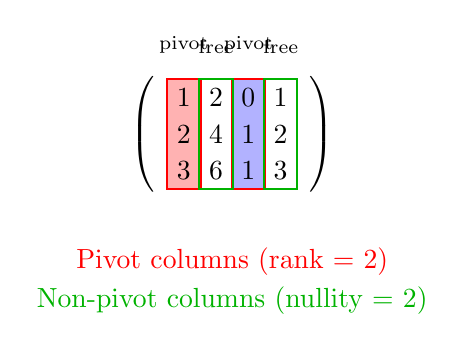
\begin{tikzpicture}[scale=0.8]
\matrix (m) [matrix of math nodes, left delimiter=(, right delimiter=), ampersand replacement=\&] {
|[fill=red!30]| 1 \& 2 \& |[fill=blue!30]| 0 \& 1 \\
|[fill=red!30]| 2 \& 4 \& |[fill=blue!30]| 1 \& 2 \\
|[fill=red!30]| 3 \& 6 \& |[fill=blue!30]| 1 \& 3 \\
};
\node[above=0.2cm of m-1-1] {\scriptsize pivot};
\node[above=0.2cm of m-1-2] {\scriptsize free};
\node[above=0.2cm of m-1-3] {\scriptsize pivot};
\node[above=0.2cm of m-1-4] {\scriptsize free};

\draw[red, thick] (m-1-1.north west) rectangle (m-3-1.south east);
\draw[red, thick] (m-1-3.north west) rectangle (m-3-3.south east);
\node[below=0.5cm of m, red] {Pivot columns (rank = 2)};

\draw[green!70!black, thick] (m-1-2.north west) rectangle (m-3-2.south east);
\draw[green!70!black, thick] (m-1-4.north west) rectangle (m-3-4.south east);
\node[below=1cm of m, green!70!black] {Non-pivot columns (nullity = 2)};
\end{tikzpicture}
\end{center}

\vspace{0.5em}

$$\underbrace{2}_{\text{rank}} + \underbrace{2}_{\text{nullity}} = \underbrace{4}_{n}$$

\end{frame}

\begin{frame}{Rank-Nullity Theorem}

\begin{thm}[Rank-Nullity Theorem]
For any $m \times n$ matrix $\underbrace{A}_{m \times n}$:

$$\boxed{\text{rank}(A) + \dim(\text{Null}(A)) = n}$$
\end{thm}

\vspace{1em}

\x{Proof idea}: Every column is either:
\begin{itemize}
\item A pivot column (contributes to rank), or
\item A non-pivot column (contributes one free variable to nullity)
\end{itemize}

Total = $n$ columns.

\end{frame}

% ═══════════════════════════════════════
% §6 ORTHOGONALITY PREVIEW
% ═══════════════════════════════════════
\section{Preview: Null Space and Row Space Orthogonality}

\begin{frame}{Natural Orthogonality}

\begin{thm}
$\text{Null}(\underbrace{A}_{m \times n}) \perp \text{Row}(\underbrace{A}_{m \times n})$

Every vector in $\text{Null}(A)$ is orthogonal to every vector in $\text{Row}(A)$.
\end{thm}

\vspace{1em}

\x{Proof}: Let $\mathbf{x} \in \text{Null}(A)$ and $\mathbf{r}_i$ = $i$-th row of $A$.

By definition: $A\mathbf{x} = \mathbf{0}$ means $\mathbf{r}_i \cdot \mathbf{x} = 0$ for all $i$.

$\Rightarrow$ $\mathbf{x} \perp$ every row $\Rightarrow$ $\mathbf{x} \perp \text{Row}(A)$. \qed

\end{frame}

\begin{frame}{Coffee Shop Interpretation}

If $\underbrace{A}_{m \times n}$ = ``drinks $\to$ ingredients'':

\begin{itemize}
\item \textbf{Row space}: All ingredient combinations from drinks
\item \textbf{Null space}: Relationships between drinks (which can be made from others)
\end{itemize}

\vspace{1em}

\x{Perpendicular}: A relationship (which drinks are equivalent) has nothing in common with actual ingredient requirements!

\vspace{1em}

\x{Next lecture}: Four fundamental subspaces and complete orthogonal structure.

\end{frame}

% ═══════════════════════════════════════
% §7 SUMMARY
% ═══════════════════════════════════════
\section{Summary}

\begin{frame}{What We Achieved Today}

\x{1. Concrete Example First}:
\begin{itemize}
\item Started with coffee shop null space problem
\item Solved completely using cross-filling before defining theory
\end{itemize}

\vspace{0.5em}

\x{2. Extracted Theory}:
\begin{itemize}
\item Null space definition from the example
\item Cross-filling method: each $(R_i \mid \mathbf{b}_i)$ = one equation
\item Variables decrease $\to$ backward solving
\item $V$ matrix and left cancellation
\end{itemize}

\vspace{0.5em}

\x{3. Applied to General Equations}:
\begin{itemize}
\item Existence: rank$(A \mid \mathbf{b})$ = rank$(A)$ $\iff$ solution exists
\item Uniqueness: $\text{Null}(A) = \{\mathbf{0}\}$ $\iff$ unique solution
\item General solution structure: $\mathbf{x} = \mathbf{x}_p + \text{Null}(A)$
\end{itemize}

\end{frame}

\begin{frame}{What We Achieved Today (continued)}

\x{4. Rank-Nullity}:

$$\text{rank}(A) + \dim(\text{Null}(A)) = n$$

Visual: pivot columns + non-pivot columns = all columns

\vspace{1em}

\x{5. Orthogonality Preview}: $\text{Null}(A) \perp \text{Row}(A)$

\vspace{1em}

\x{Next lecture}: Four fundamental subspaces and their complete orthogonal structure!

\end{frame}

\end{document}
